\subsection{Mathematical Models for Time Series}
\subsubsection{Mathematical Concepts of Time Series}
{
	\begin{figure}[H]\centering
		\begin{minipage}[c]{0.5\textwidth}
			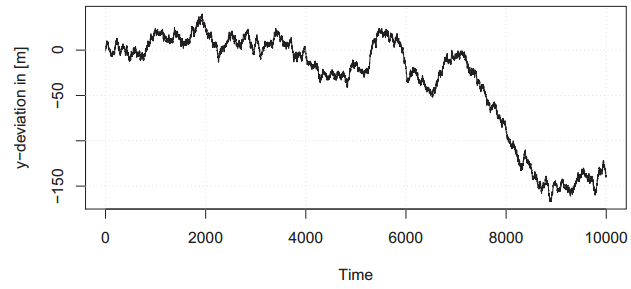
\includegraphics[width=1\linewidth]{images/randomWalk.png}
			\subcaption{Random walk process}
			\label{Fig:raWa}
		\end{minipage}\hfill
		\begin{minipage}[c]{0.5\textwidth}
			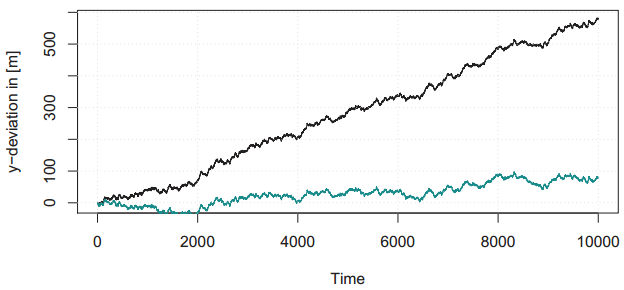
\includegraphics[width=1\linewidth]{images/randomWalkDrift.png}
			\subcaption{Random walk with drift (black) }
			\label{Fig:raWaDrift}
		\end{minipage}
	\caption{Time series observation of a random walk process}
	\end{figure}

	\RTheory
	{\textbf{Time series and discrete stochastic process}
		\begin{enumerate}
			\item A \textit{discrete stoachstic process} is a set of random variables $\{X_1, X_2, . . . \}$. Each single random variable $X_i$ has a univariate distribution function $F_i$ and can be observed at time $t_i$.
			\item A \textit{time series} $\{x_1, x_2, . . .\}$ is a realization of a discrete stochastic process $\{X_1, X_2, . . . \}$. In other words, the value $x_i$ is a realization of the random variable $X_i$ measured at time $t_i$.
		\end{enumerate}
	}
	{sections/TimeSeriesAnalysis/MathematicalModelsForTimeSeries/RCode/tsMathConc.R}
\RTheory
{\textbf{White noise processes}\vfill
A white noise process consists of i.i.r. variables $\{W_1,W_2,...\}$ where $W_i$ has mean $0$ and variance $\sigma^2$.
\vfill
\hfill
\break
If we apply a sliding window filter to the white noise process $\{W_1, W_2,...\}$ we obtain a \textit{moving average process}. With a window length of 3 we obtain
$$V_i =\frac{1}{3}(W_{i-1}+W_{i}+W_{i+1})$$.
\vfill
\hfill
\break
Considering again the white noise process, computing the following sequence
$$X_i = 1.5X_{i-1}-0.9X_{i-2}+W_i $$
The value of the process at time instance $i$ is modelled as linear combination of the past two values plus some random component. This process is called \textit{autoregressive}.
}
{sections/TimeSeriesAnalysis/MathematicalModelsForTimeSeries/RCode/tsWhiteNoise.R}
\begin{figure}[H]\centering
	\begin{minipage}[c]{0.5\textwidth}
		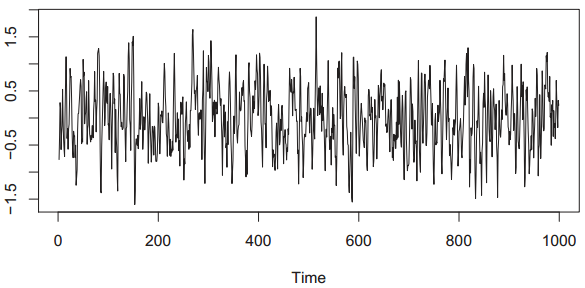
\includegraphics[width=1\linewidth]{images/whNoMovAv.png}
		\subcaption{Moving average process of white noise}
		\label{Fig:whNoMA}
	\end{minipage}\hfill
	\begin{minipage}[c]{0.5\textwidth}
		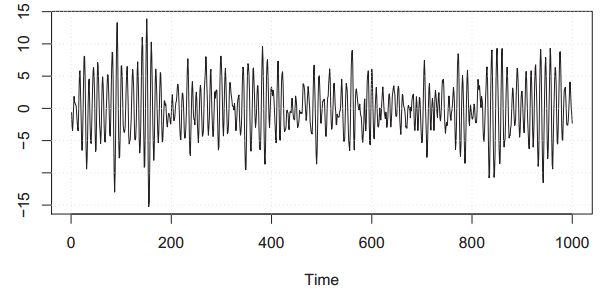
\includegraphics[width=1\linewidth]{images/whNoAR.png}
		\subcaption{Autoregressive process of white noise}
		\label{Fig:whNoAR}
	\end{minipage}
\end{figure}
}
\subsubsection{Measures of Dependence}
{
	
	\begin{twoColTable}
	\hline
	\rowcolor{HSRBlue40}\textbf{Autocovariance and autocorrelation}
	& \textbf{Example}\\
	\hline
	Let $\{X_1,X_2,...\}$ be a discrete stochastic process
	\begin{enumerate}
		\item The \textit{autocovariance} $\gamma_X$ is defined as
		$$\gamma_X(i,j)=Cov(X_i,X_j)= E[(X_i-\mu(i))(X_j-\mu(j))]	$$
		\item The \textit{autocorrelation} $\rho_X$ is defined as
		$$ \rho_X(i,j)=\frac{\gamma_X(i,j)}{\sqrt{\gamma_X(i,i)\gamma_X(j,j)}}$$
	\end{enumerate}
		Note that the autocovariance and the autocorrelatiion are symmetric, i.e. $\gamma(i,j)=\gamma(j,i)$. The autocovariance measures the \textit{linear dependence} of two points on the same process observed at different times. For $i=j$ the autocovariance reduces to the variance of $X_i$.\vfill
		\hfill
		\break
		The autocorrelation hence gives a rough measure how well the series at time $i$ can be forecast by the value at time $j$.
		\vfill
		\hfill
		\break
		It is important to consider the properties of the process model. For example a white noise process has the autocovariance function
		$$
		\gamma(i,j)=
		\begin{cases}
		0 & i\neq j\\
		\sigma^2 & i = j
		\end{cases}
		$$
		Accordingly the autocorrelation is 1 if $i=j$ and 0 else.
	& 
	The autocovariance of the three point moving average process is computed as follows.\vfill
	{\centering	$\gamma(i,j)=Cov(X_i,X_j)=$\vfill} {\centering	$Cov\bigg(\frac{1}{3}(W_{i-1}+W_i+W_{i+1}),\frac{1}{3}(W_{j-1}+W_j+W_{j+1})\bigg) $\vfill}
	When $i=j$\vfill
	{\centering$Cov(X_i,X_i)=\frac{1}{9}Cov(W_{i-1}+W_i+W_{i+1},W_{i-1}+W_i+W_{i+1})$\vfill}
	{\centering$=\frac{1}{9}(Cov(W_{i-1},W_{i-1})+Cov(W_{i},W_{i})+Cov(W_{i+1},W_{i+1}))$\vfill}
	{\centering$=\frac{3\sigma^2}{9}$\vfill}
	This follows from the fact, that $W_i,W_{i-1}$ and $W_{i+1}$ are \textit{mutually uncorrelated}. For $i+1 = j$ we find\vfill
	{\centering$Cov(X_i,X_{i+1})=\frac{1}{9}Cov(W_{i-1}+W_i+W_{i+1},W_{i}+W_{i+1}+W_{i+2})$\vfill}
	{\centering$=\frac{1}{9}(Cov(W_{i},W_{i})+Cov(W_{i+1},W_{i+1}))=\frac{2\sigma^2}{9}$\vfill}
	Summarized:\vfill
	$$ \gamma(i,j)=
	\begin{cases}
	\frac{3\sigma^2}{9} & i=j\\
	\frac{2\sigma^2}{9} & |i-j|=1\\
	\frac{\sigma^2}{9} & |i-j|=2\\
	0					& else
	\end{cases}
	$$
	In this example the autocovariance only depends on the distance of the observations, but not on their value. Hence the autocorrelation $\rho(i,j)=\gamma(i,j)/\sqrt{\gamma(i,i)\gamma(j,j)}=\gamma(i,j)/\gamma(i,i)$
	This gives\vfill
	$$ \rho(i,j)=
	\begin{cases}
	1 & i=j\\
	\frac{2}{3} & |i-j|=1\\
	\frac{1}{3} & |i-j|=2\\
	0					& else
	\end{cases}
	$$
	\\
	\hline
\end{twoColTable}
\begin{twoColTable}
	\hline
	\rowcolor{HSRBlue40}\textbf{Mean sequence (or mean function)}
	& \textbf{Example}\\
	\hline
	The mean sequence $\{\mu(1),\mu(2),...\}$ of a discrete stochastic process $\{X_1,X_2,...\}$ is defined as the sequence of the means: 
	$$\mu(i) = E[X_i].$$
	& 
	If $X_i$ is a random walk with drift, i.e. $X_0$ and $X_i =\delta + X_{i-1} +W_i$ then we find that 
	$$E[X_1]=\delta + E[X_0] + E[W_1] = \delta$$
	$$E[X_2]=\delta + E[X_1] + E[W_2] = 2\delta$$
	$$E[X_3]=\delta + E[X_2] + E[W_3] = 3\delta$$
	$$etc.$$
	This means that $\mu(i) = i\delta$.
	\\
	\hline

\end{twoColTable}
}
\subsubsection{Stationarity}
{
Stationarity is a concept of regularity that allows us to infer information from a single time series.

\begin{twoColTable}
	\hline
\rowcolor{HSRBlue40}\textbf{Strict stationarity}
& \textbf{Weak stationarity}\\
\hline
	A discrete stochastic process is called strictly stationary if for each finite collection $\{X_{i_1}, . . . , X_{i_n}\}$ and each lag $h \in \mathbb{Z}$ the shifted collection
$$ \{X_{{i_1}+h}, . . . , X_{{i_n}+h}\} $$
has the \textbf{same distribution}. Put differently
$$ P(X_{i_1} \leq c_1,...,X_{i_n} \leq c_n)=P(X_{{i_1}+h} \leq c_1,...,X_{{i_n}+h} \leq c_n)$$
This means that the probabilistic character of the process does not change over time. For many applications is strict stationarity a too strong assumption and hard to assess from a single data set.
&
A discrete stochastic process $X_i$ is called \textit{weakly stationary} if
\begin{enumerate}
	\item the mean sequence $\mu_X(i)$ is constant and does not depend on the time index $i$ and
	\item the autocovariance sequence $\gamma_X(i,j)$ depends on $i$ and $j$ only through their difference $|i-j|$.
\end{enumerate}
Each strictly stationary time series is also weakly stationary. But the opposite is in general not true.
\vfill
\hfill
\break
Since the autocovariance/-correlation for a (weakly) stationary process only depends on the {\textbf{time \textit{lag} $h=i-j$}} one considers these sequences as a function of $h$ alone:
$$ 
\gamma(h)=\gamma(i,i+h)
$$
$$
\rho(h)=\rho(i,i+h)
$$
See also the example of the moving average process above.
\\
\hline
\end{twoColTable}
\paragraph{Testing Stationarity}
\begin{figure}[H]\centering
	\begin{minipage}[c]{0.5\textwidth}
		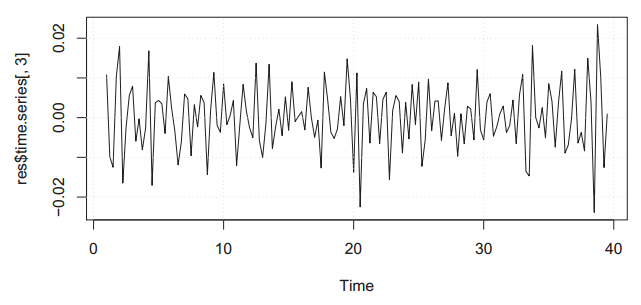
\includegraphics[width=1\linewidth]{images/tsAusElRemainder.png}
		\subcaption{Remainder: Australian Electricity}
		\label{Fig:tsAusElRem}
	\end{minipage}\hfill
	\begin{minipage}[c]{0.5\textwidth}
		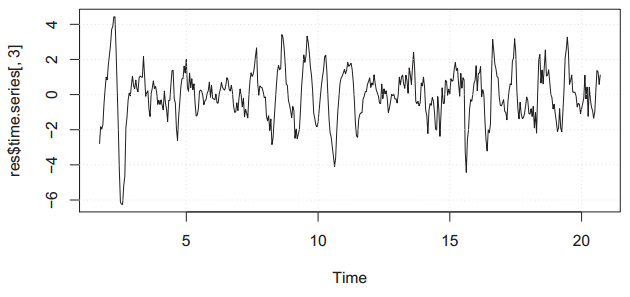
\includegraphics[width=1\linewidth]{images/tsAirTempRemainder.png}
		\subcaption{Remainder: Air Temperature}
		\label{Fig:tsAirTempRem}
	\end{minipage}
\caption{Testing stationarity}
\end{figure}
\RTheory
{
In practice we have to \textit{test} or at least \textit{guess} whether or not the underlying process of a given time series is stationary.
There are several statistical hypothesis test for stationarity. 
\vfill
\hfill
\break
The first and simplest test one can apply to check for stationarity is to plot the time series and look for evidence of trend in mean, variance, autocorrelation and seasonality. If such patterns are present then these are signs of non-stationarity and different mechanism exit to turn the series into a stationary one, as data transformation or time series decomposition.
\vfill
\hfill
\break
A further possibility is to compute the mean and autocovariance sequences seperately for several windows and compare their behaviour. When there is a dramatic change, then the hypotheses of stationarity can be rejected.
\vfill
\hfill
\break
The series in Figure \ref{Fig:tsAusElRem} does not exhibit any seasonal patterns, has a constant mean and roughly constant variance. From visual inspection one would conclude that the underlying process is stationary.
\vfill
\hfill
\break
The series in Figure \ref{Fig:tsAirTempRem} still exhibits some seasonality, such that stationarity of the underlying process seems unlikely.
}
{sections/TimeSeriesAnalysis/MathematicalModelsForTimeSeries/RCode/tsTestingStationarity.R}
}
\subsubsection{Estimation of Correlation}
{
In this section it is assumed that the time series $\{x_1,x_2,...,x_n\}$ is a realization of a weakly stationary process $\{X_1,X_2,...,X_n\}$.
\begin{figure}[H]\centering
	\begin{minipage}[c]{0.5\textwidth}
		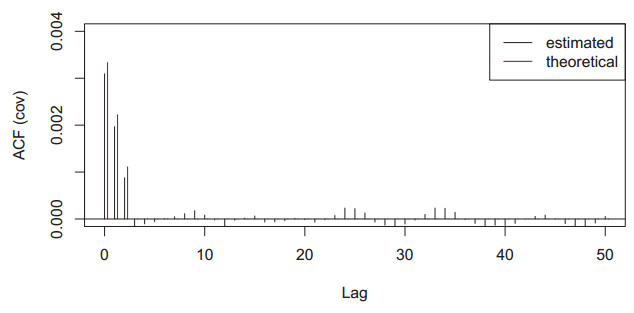
\includegraphics[width=1\linewidth]{images/tsCov.png}
		\subcaption{Sample autocovariance function of a MA(5) process (black) and the theoretical values (red)}
		\label{Fig:tsSamAutoCov}
	\end{minipage}\hfill
	\begin{minipage}[c]{0.5\textwidth}
		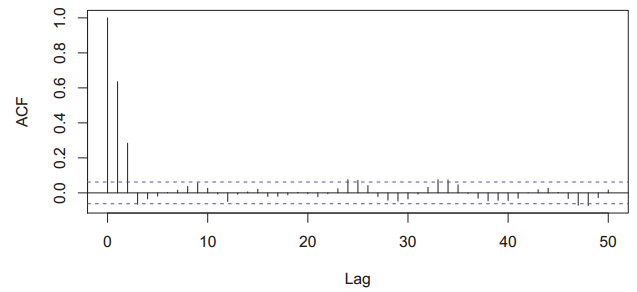
\includegraphics[width=1\linewidth]{images/tsACF.png}
		\subcaption{Sample autocorrelation function of MA(5) process}
		\label{Fig:tsSamAutoCor}
	\end{minipage}
	\caption{Estimation of Correlation}
\end{figure}
\RTheory
{\textbf{Estimation of the mean sequence}\vfill
Due to stationarity we know that the mean sequence $\mu(k)=\mu$ is constant. A canonical estimator hence is 
$$\hat{\mu}=\bar{x}=\frac{1}{n}\sum\limits_{i=1}\limits^{n}x_i$$
In the present situation the observations are dependent. Hence the standard error $\sigma/\sqrt{n}$ is not applicable. We have to recompute the standard error.
$$Var(\hat{\mu})=\frac{1}{n}\sum\limits_{h=-n}\limits^{n}\bigg(1- \frac{|h|}{n}\bigg)\gamma(h) $$
\vfill
\hfill
\break
\textbf{Estimation of the autocovariance}\vfill
The theoretical autocovariance function is estimated by the sample autocovariance sequence which we define as

\begin{enumerate}
	\item The \textit{sample autocovariance} is defined by
	$$\hat{\gamma}(h)= \frac{1}{n} \sum\limits_{i=1}\limits^{n-h}(x_{i+h}-\hat{x})(x_i-\bar{x})$$ 
	with $\hat{\gamma}(h)=\hat{\gamma}(-h)$ for $h=0,1,...,n-1$
	\item The \textit{sample autocorrelation} is defined by
	$$\hat{\rho}=\frac{\hat{\gamma}(h)}{\hat{\gamma}(0)} $$
\end{enumerate}
Note that the sum runs over a restricted range of $n-h$ points but we nevertheless normalize by $n$ rather than $n-h$. Neither choice results in an unbiased estimator.
}
{sections/TimeSeriesAnalysis/MathematicalModelsForTimeSeries/RCode/tsEstimCorr.R}


}